\documentclass{scrartcl}
\usepackage[utf8]{inputenc}
\usepackage[english]{babel}
\usepackage{caption}
\usepackage{subcaption}
\usepackage{listings}
\usepackage{pdfpages}
\usepackage{amsmath,amssymb}
\usepackage{siunitx}
\usepackage{hyperref}
\usepackage{mhchem}
\usepackage[section]{placeins}
\usepackage[activate, protrusion=true, expansion=true]{microtype}
\usepackage[left=2.5cm, right=2.5cm, bottom=2.5cm, top=2.5cm]{geometry}
\usepackage{libertine}
\usepackage{longtable}

\definecolor{mygreen}{rgb}{0,0.6,0}
\definecolor{mymauve}{rgb}{0.58,0,0.82}
\definecolor{mygray}{rgb}{0.5,0.5,0.5}
\lstset{backgroundcolor=\color{white},
  keepspaces=true,
  captionpos=b,
  keywordstyle=\color{blue},
  language=matlab,
  stringstyle=\color{mymauve},
  tabsize=2,
  numbers=left,                    % where to put the line-numbers; possible values are (none, left, right)
  numbersep=5pt,                   % how far the line-numbers are from the code
  numberstyle=\tiny\color{mygray},
  basicstyle=\footnotesize,        % the size of the fonts that are used for the code
  breakatwhitespace=false,         % sets if automatic breaks should only happen at whitespace
  breaklines=true,                 % sets automatic line breaking
  commentstyle=\color{mygreen},    % comment style
  deletekeywords={input},            % if you want to delete keywords from the given language
}

\newcommand*{\matlabcode}[3]{\begin{figure}[h!]\lstinputlisting[caption=#2, label=#3]{#1}\end{figure}}


\usepackage{scrpage2}
\pagestyle{scrheadings}
\automark{section}
\ihead{\rightmark}
\chead{}
\ohead{
\includegraphics[scale=0.025]{figures/EPFL_Logo.png}}
\setheadsepline{.4pt}

\begin{document}

\begin{titlepage}

\title{CE-2: Parametric Identification Methods} % Title
\author{Arne Sachtler \\ Julia Krottenthaler}		% Author
\date{\today}								% Date

\makeatletter
\let\thetitle\@title
\let\theauthor\@author
\let\thedate\@date
\makeatother

\centering
\vspace*{0.5 cm}

    
\includegraphics[width=0.7\linewidth]{figures/EPFL_Logo.png}\\[1.0 cm]	
	\textsc{\Large System Identification (ME-421)}\\[1.0cm]				
	\rule{\linewidth}{0.2 mm} \\[0.5 cm]
	{ \LARGE \thetitle}\\
	\rule{\linewidth}{0.2 mm} \\[1.5 cm]
	
    \vspace{1cm}
	\begin{minipage}{0.5\textwidth}
		\begin{flushleft} \large
			\emph{{Students}:}\\
			\theauthor
			\end{flushleft}
			\end{minipage}~
			\begin{minipage}{0.4\textwidth}
			\begin{flushright} \large
			\emph{{Lecturer}:} \\	
			Prof. Karimi Alireza  \\
		\end{flushright}
	\end{minipage}\\[1.2cm]
	{\vspace{3cm} \large Lausanne, \thedate}\\[1.5 cm]
	\vfill
\end{titlepage}

\tableofcontents

\newpage
\section{Identification of a Laser Beam Stabilizing System}

\subsection{FIR Model Identification}\label{sec:FIR}

In this section we identify a finite impulse response (FIR) model using the time-domain data \texttt{laserbeamdataN.mat}. This file contains the input $u$ and the output signal $y$ of a laser beam stabilizing system shown in Figure~\ref{fig:system} with a set of $ N = 500 $ data.  

\begin{figure}[h]
	\centering
	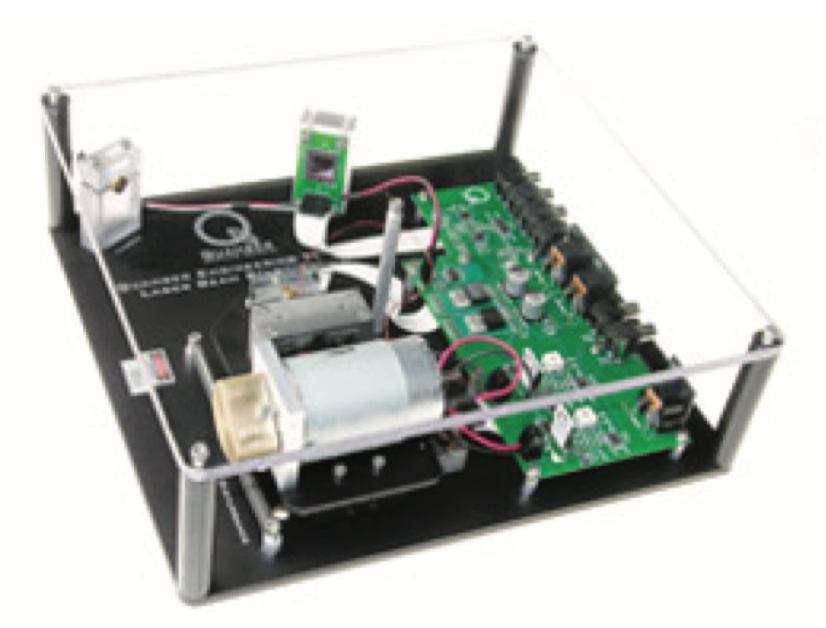
\includegraphics[height=4cm]{figures/system.png}
	\caption{Laser beam stabilizing system }\label{fig:system}
\end{figure}

We assume a FIR model of the following form:
\begin{equation}\label{eq:FIRmodel}
	\hat{y}(k,\theta) = b_1 u(k-1) + \cdots + b_m u(k-m) \qquad m = 1,2,\ldots,50.
\end{equation}

This model can be rewritten as follows:

\begin{align}\label{eq:FIRrewritten}
	 \hat{y} (k,\theta) & = \phi^{T} (k) \theta 
 \intertext{where}
 	 \phi^{T} (k) & = \left[ u(k-1), u(k-2), \ldots, u(k-m) \right] \\
 	 \theta^T & = \left[ b_1, b_2, \ldots, b_m \right] .
\end{align}

First, we compute the parameter vector $\hat{\theta}$ using the least squares algorithm and the Moore-Penrose pseudo inverse $\pmb{\phi}^+$ of $\pmb{\phi}$:

\begin{equation}\label{eq:FIRmodel}
	\hat{\theta} = \left[ \sum\limits_{k=1}^N \phi(k)\phi^T(k) \right]^{-1} \sum\limits_{k=1}^N 
\phi(k) y(k) = \left( \pmb{\phi}^T \pmb{\phi} \right)^{-1} \pmb{\phi}^T \textbf{Y} = \pmb{\phi}^+ \textbf{Y}.
\end{equation}

Here, $\pmb{\phi}$ is an asymmetric (lower) triangular Toeplitz matrix, which we generate with the MATLAB \texttt{toeplitz} command.
In MATLAB we can solve this least squares problem by simply using the backslash operator. 

Afterwards, we compute the predicted output of our identified model $\hat{y} (k,\hat{\theta}) = \phi^{T} (k) \hat{\theta}$. The result can be seen in Figure~\ref{fig:output_fir}.

\begin{figure}[h]
	\centering
	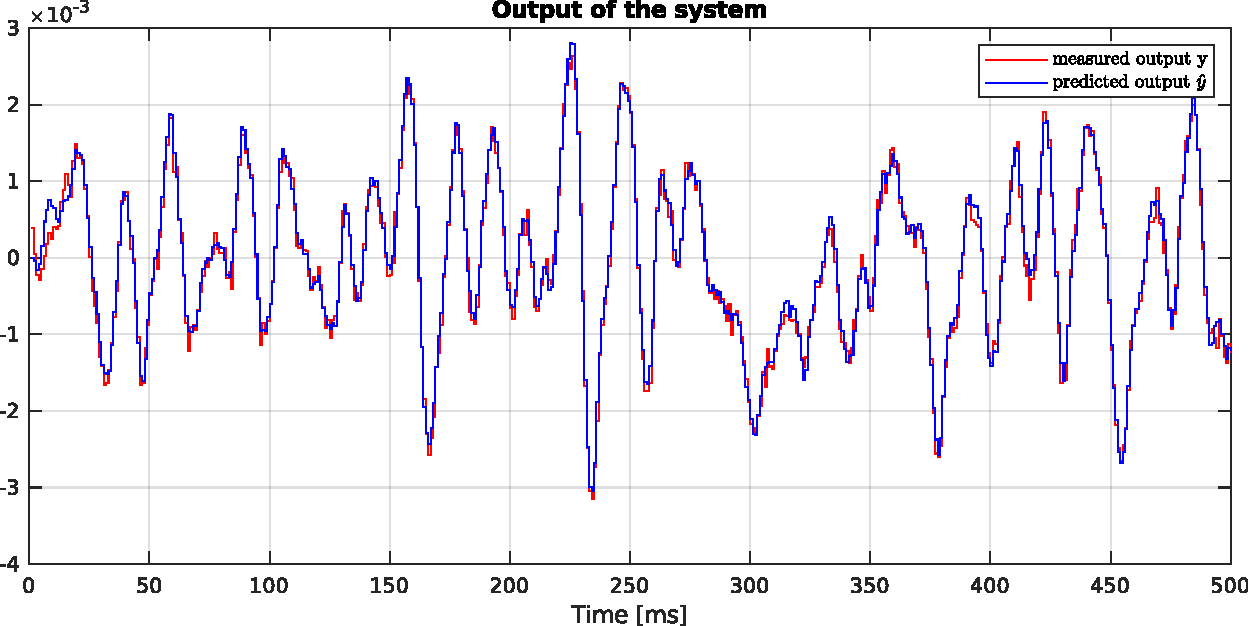
\includegraphics[height=5.5cm]{figures/output.pdf}
	\caption{Output of the system}\label{fig:output_fir}
\end{figure}

In order to estimate the quality of our predictor, we need a fit criterion, which should minimised. We therefore consider a loss function as 
\begin{equation}\label{eq:J}
	J(\theta) = \sum\limits_{k=1}^N \left[y(k) - \hat{y}(k,\theta) \right]^2.
\end{equation}
Using the MATLAB command \texttt{norm} and squaring the result we obtain $ J(\theta) \approx 6.92 \cdot 10^{-6}$. 

As we assume that the noise is white, we obtain an unbiased estimate of the noise variance by
\begin{equation}\label{eq:sigma}
	\hat{\sigma}_{noise}^{2} = \frac{1}{N-m} J(\hat{\theta}) .
\end{equation}

Using the available data this equation yields to $ \hat{\sigma}_{noise} \approx 1.24 \cdot 10^{-4} $.

The covariance of the parameter estimates can then be obtained as
\begin{equation}\label{eq:cov}
	cov[\hat{\theta}] = \hat{\sigma}_{noise}^2 \left[ \sum\limits_{k=1}^N \phi(k)\phi^T(k) \right]^{-1} = \hat{\sigma}_{noise}^2 \left( \pmb{\phi}^T \pmb{\phi} \right)^{-1} .
\end{equation}

The square root of the diagonal elements of the $cov[\hat{\theta}]$ matrix is the standard deviation $ \sigma $, which we use for the $ \pm 2 \sigma $ confidence interval in Figure~\ref{fig:fir_response}. This figure shows us the finite impulse response of the system.

\begin{figure}[h]
	\centering
	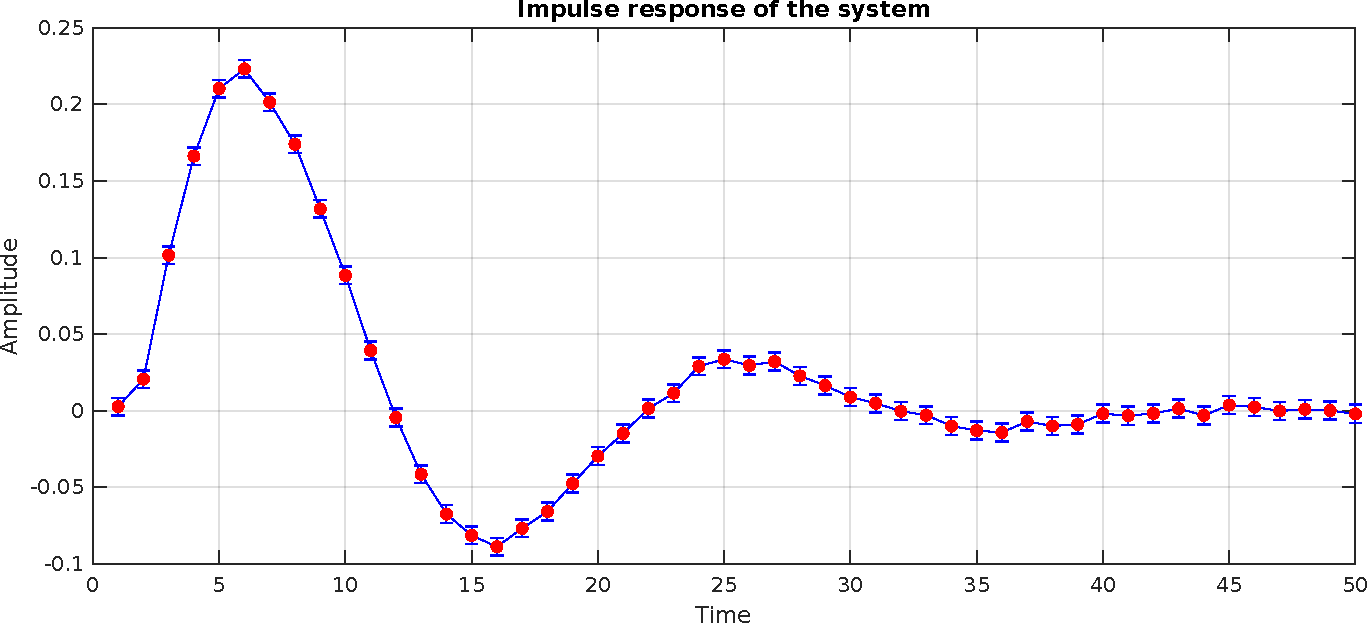
\includegraphics[height=5.5cm]{figures/fir_response.pdf}
	\caption{Finite impulse response of the system}\label{fig:fir_response}
\end{figure}

\matlabcode{../matlab/ce2/FIR_model_identification.m}{Computing the finite impulse response of the system}{lst:FIR}

\clearpage


\newpage
\subsection{ARX Model Identification}
We now assume a second order auto-regressive with external input (ARX) model for the same data as in the previous chapter (\texttt{laserbeamdataN.mat}, $N = 500$). Therefore, we use the following predictor
\begin{align}\label{eq:arx}
	\hat{y}(k,\theta) & = -a_1 y(k-1) - a_2 y(k-2) + b_1 u(k-1) + b_2u (k-2) = \phi^T(k) \theta
	\intertext{where}
 	 \phi^{T} (k) & = \left[ -y(k-1), -y(k-2), u(k-1), u(k-2) \right] \\
 	 \theta^T & = \left[ a_1, a_2, b_1, b_2\right] .
\end{align}
We observe that the system has no modeled delay as $d = 0$.
Using the least squares algorithm and the Moore-Penrose pseudo inverse $\pmb{\phi}^+$ of $\pmb{\phi}$, we compute, like we did it already in Section~\ref{sec:FIR}, the parameter vector $\hat{\theta}$:
\begin{equation}\label{eq:ARXmodel}
	\hat{\theta} = \left[ \sum\limits_{k=1}^N \phi(k)\phi^T(k) \right]^{-1} \sum\limits_{k=1}^N 
\phi(k) y(k) = \left( \pmb{\phi}^T \pmb{\phi} \right)^{-1} \pmb{\phi}^T \textbf{Y} = \pmb{\phi}^+ \textbf{Y}.
\end{equation}
In order to estimate the quality of our predictor, we need a fit criterion, which should minimised. Hence, we consider a loss function as 
\begin{equation}\label{eq:J}
	J(\theta) = \sum\limits_{k=1}^N \left[y(k) - \hat{y}(k,\theta) \right]^2.
\end{equation}
We construct the matrix consisting of the input and output values according to the predictor structure and solve for the parameters using the backlash operator.
Using this, we obtain $ J(\theta) \approx 2.17 \cdot 10^{-5}$. 
The predicted output of our identified model $\hat{y}(k,\hat{\theta})$ is then computed using 
$\hat{y}(k,\hat{\theta}) = \phi^{T} (k) \hat{\theta}$. The result can be seen in Figure~\ref{fig:output_arx}.
Note that this predictor (in contrast to the simulated transfer function below) uses the measured past value of the output.

\begin{figure}[h]
	\centering
	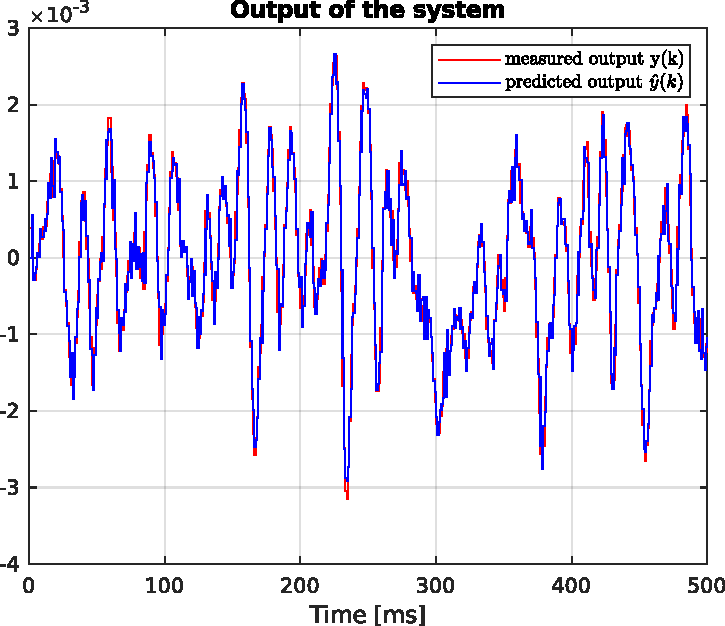
\includegraphics[height=5.5cm]{figures/output_arx.pdf}
	\caption{Output of the identified ARX model compared to the measured output }\label{fig:output_arx}
\end{figure}

Afterwards we compute the output of the identified model $y_m(k)$ using the MATLAB command \texttt{lsim}. On that point, we generate a transfer function with the MATLAB command \texttt{tf}. Thus, the obtained output $y_m(k)$ compared to the measured output $y(k)$ can be seen in Figure~\ref{fig:output_lsim2}.
The resulting sum of the squares of the error is then $ J(\theta) \approx 1.14 \cdot 10^{-4}$. 

\begin{figure}[h]
	\centering
	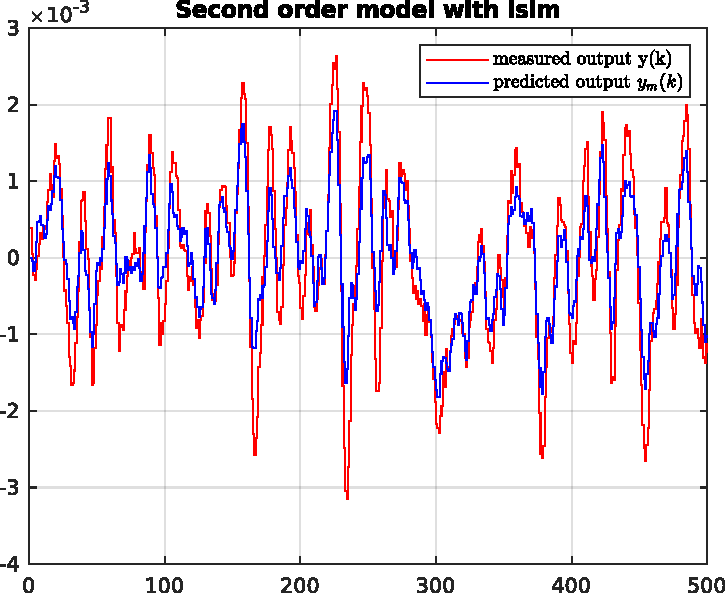
\includegraphics[height=5.5cm]{figures/output_lsim2.pdf}
	\caption{Output of the second order \texttt{lsim} model compared to the measured output}\label{fig:output_lsim2}
\end{figure}



It is remarkable that the value of the output of the identified model is much smaller than the measured output. In order to achieve better results, we raise the order of our model to $3$, with

\begin{align}\label{eq:arx}
 	 \phi^{T} (k) & = \left[ -y(k-1), -y(k-2), -y(k-3), u(k-1), u(k-2), u(k-3) \right] \\
 	 \theta^T & = \left[ a_1, a_2, a_3, b_1, b_2, b_3\right] .
\end{align}

This model approaches the real output values much better, as it can be seen in Figure \ref{fig:output_lsim3}.

\begin{figure}[h]
	\centering
	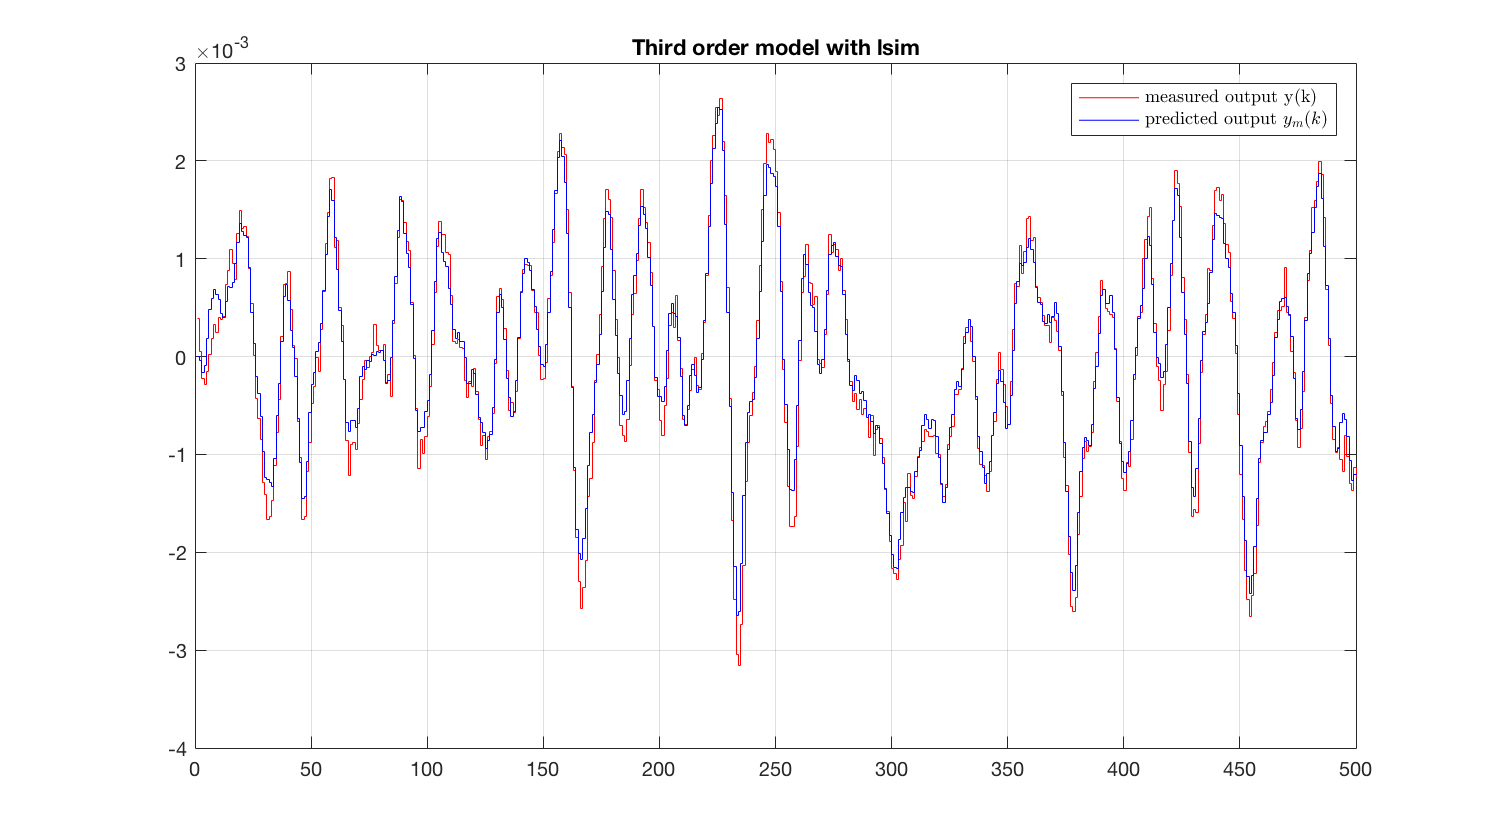
\includegraphics[height=5.5cm]{figures/output_lsim3.png}
	\caption{Output of the third order \texttt{lsim} model compared to the measured output}\label{fig:output_lsim3}
\end{figure}

\newpage
\subsection{State-space Model Identification}

\newpage
\section{Parametric Identification of an Active Suspension System}

\newpage
\subsection{Order Estimation}

\newpage
\subsection{Parametric Identification}

\newpage
\subsection{Model Validation}
\end{document}
